
\documentclass[a4paper]{article}
\usepackage[margin=1in]{geometry}
\usepackage[english]{babel}
\usepackage[utf8]{inputenc}
\usepackage{amsmath,amsthm,amssymb}
\usepackage{graphicx}
\usepackage{epstopdf}
\usepackage{pdfpages}
\usepackage{float, algorithmic, algorithm2e, program}
\usepackage{tabularx}
\usepackage{longtable}
\usepackage{epstopdf}
\newtheorem{theorem}{Theorem}
\newtheorem{definition}{Definition}[section]

\title{Bathtub Qualitative Reasoning}
\author{Nicola De Cao, Luca Falorsi, Govert Verkes}
\date{\today}

\begin{document}
\maketitle

\section{Base Problem}

\begin{itemize}
\item \textbf{Quantities:}
\begin{itemize}
\item Inflow (of water into the container) $\in [0, +]$
\item Outflow (of water out of the container) $\in [0, +, Max]$
\item Volume (of the water in the container) $\in [0, +, Max]$
\end{itemize}

\item \textbf{Dependencies:}

\begin{itemize}
\item I+(Inflow, Volume): the amount of inflow increases the volume
\item I-(Outflow, Volume): the amount of outflow decreases the volume
\item P+(Volume, Outflow): outflow changes are proportional to volume changes
\item V(Volume(Max), Outflow(Max)): the outflow is at its highest value (Max), when the volume is at it highest value
\item V(Volume(0), Outflow(0)): there is no outflow, when there is no volume
\end{itemize}
\end{itemize}


\begin{figure}[H]
\centering
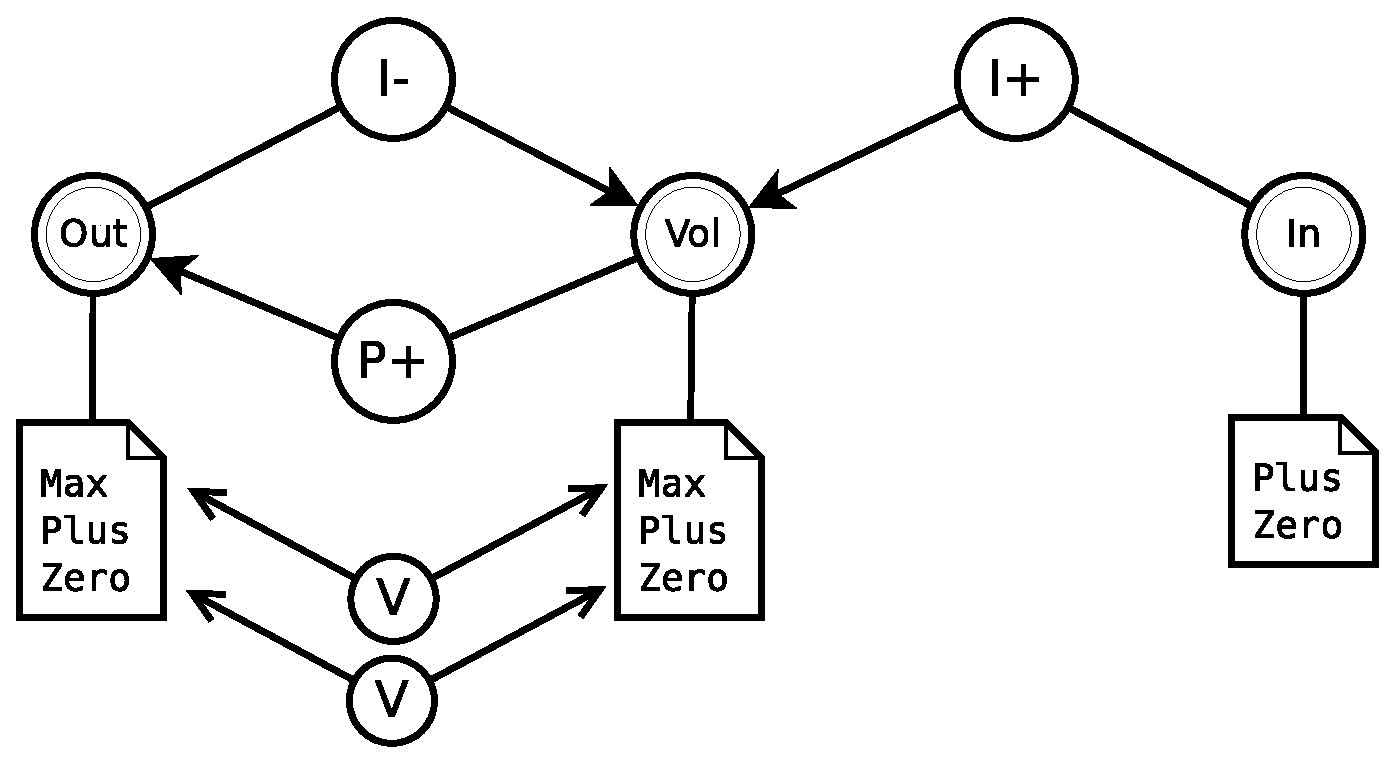
\includegraphics[scale=0.5]{problem1.eps}
\caption{Drawings of the causal model active for the problem}
\end{figure}

\section{Algorithm}
The goal of the algorithm is to construct a state graph based for a specific model and a given starting state. Constructing the state-graph is done iteratively as shown in Algorithm~\ref{alg:computing_state_graph}.
\begin{algorithm}
    result = \{"state": starting\_state, "children": [ ]\}

    processing\_list = [starting\_state]

\While{processing\_list not empty}{
    processing\_state = pop(processing\_list)

    successors = findSuccessors(processing\_state)

    \For{s in succesors}{
        \If{s not in result}{
            add s to result

            add s to processing\_list
        }
        add s as child to processing\_state
    }
}
\caption{Computing the state-graph based on given an starting state. It starts with a given starting state in the processing list, then it computes all the successors of this state and adds all the successors as children to state that is being processed, as well as adding these successors to the processing list, but only if a successor was not already processed.}
\label{alg:computing_state_graph}
\end{algorithm}

The core functionality of constructing the state graph is encapsulated in finding all successive states for a given state. The first step in finding the successive states, is propagating over all quantities in the model and computing all possible combinations of new values based on the derivatives. The algorithm for doing this is shown in Algorithm~\ref{alg:propogating_values}.
\begin{algorithm}
new\_states = [ empty\_state ]

    \For{quantity in quantities}{

        p = possible next values for quantity\\
        \ForAll{new\_states}{
            new\_state = pop(new\_states)\\
            \ForAll{p}{
               add new\_state with new possible value for quantity to new\_states
            }
        }
        }
\caption{Propagate over all quantities and modify value based on the derivative. This is done by looping over all quantities in the model and computing all the possible values for a next state based on its current value and its derivative. For each possible next value we create a new state, thus possibly creating multiple states. Because, we can have new states created by value splits of previous quantities, we need to create new states for each state that was created previously}
\label{alg:propogating_values}
\end{algorithm}

After computing all the possible successive states only with respect to the values, the algorithm performs a check whether all value constraints hold and removes the state if a state does not satisfy all value constraints.

The next step in the algorithm is to determine new derivatives based on the influences, the algorithm for doing this is shown in Algorithm~\ref{alg:propogating_influences}.
\begin{algorithm}

    \For{quantity in quantities}{

        \ForAll{new\_states}{

            new\_state = pop(new\_states)\\

            possible\_derivatives = [ ]

            \ForAll{influences on quantity}{
                \If{influence is not zero}{
                    add corresponding derivative to possible\_derivative based on new\_state
                }
            }
            \If{both positive and negative derivative are possible} {
                add 0 derivative to possible\_derivative
            }
            \If{values of influences did not change w.r.t.\ previous state} {
                set possible\_derivative only to old derivative
            }

            \ForAll{possible\_derivatives}{
                add new state to new\_states with new possible derivative
            }

        }

    }
\caption{Compute the new possible derivatives based on the influences. For all new states created from the previous step (value propagation), generate a list of possible derivatives. Then if both derivatives are possible this implies ambiguity and the 0 derivative is also a possibility. If the values of the influences in the previous state did not change this means that the derivative also does not change (w.r.t.\ the influences). Finally, for each state we create multiple new states based on the possible derivatives.}
\label{alg:propogating_influences}
\end{algorithm}

The last step in the algorithm is computing the new derivatives based on the proportionalities. Again we loop over all the quantities in the model. Then, for each quantity we check the derivatives of the quantities it is proportional to. If a quantity it is proportional to, has itself a quantity it is proportional to, we check these quantities first, this is implemented as a recursive algorithm. If the algorithm reaches a quantity that has not proportionalities or influences, we base its derivative on an extrogeneous influence (random). On the other hand, if the algorithm reaches a quantity that only has influences, then we know that the derivative of this quantity is already determined in the previous step (propogating the influences) and thus we do not have to go deeper into recursion. In order to prevent the algorithm from entering an infinite loop (due to cycles in the influences graph), we keep track of the quantities we visited and stop visiting them again.

When we found possible derivatives for each quantity based on its proportionalities, we create new states for each new state that was created by the previous propogations (value, value constraints and influences). All the propogations steps together leave us with possible next states. Which are passed to the iterative algorithm for construction a state-graph (Algorithm~\ref{alg:computing_state_graph}).

\section{State-graph}
The algorithm explained in the previous section generates a list of states, with children relations explaining the successor relations. Besides normal state transitions, we also have state transition due to extrogeneous influence. For this problem the only external influence we allow is changing the derivative of the Inflow randomly.

In figure \ref{state-graph} shows all possible behaviors of the system described above. Blue nodes are final states, which are states without other reachable states. Other nodes are red and each arrow represents a transition.

\begin{figure}\label{state-graph}
\centering
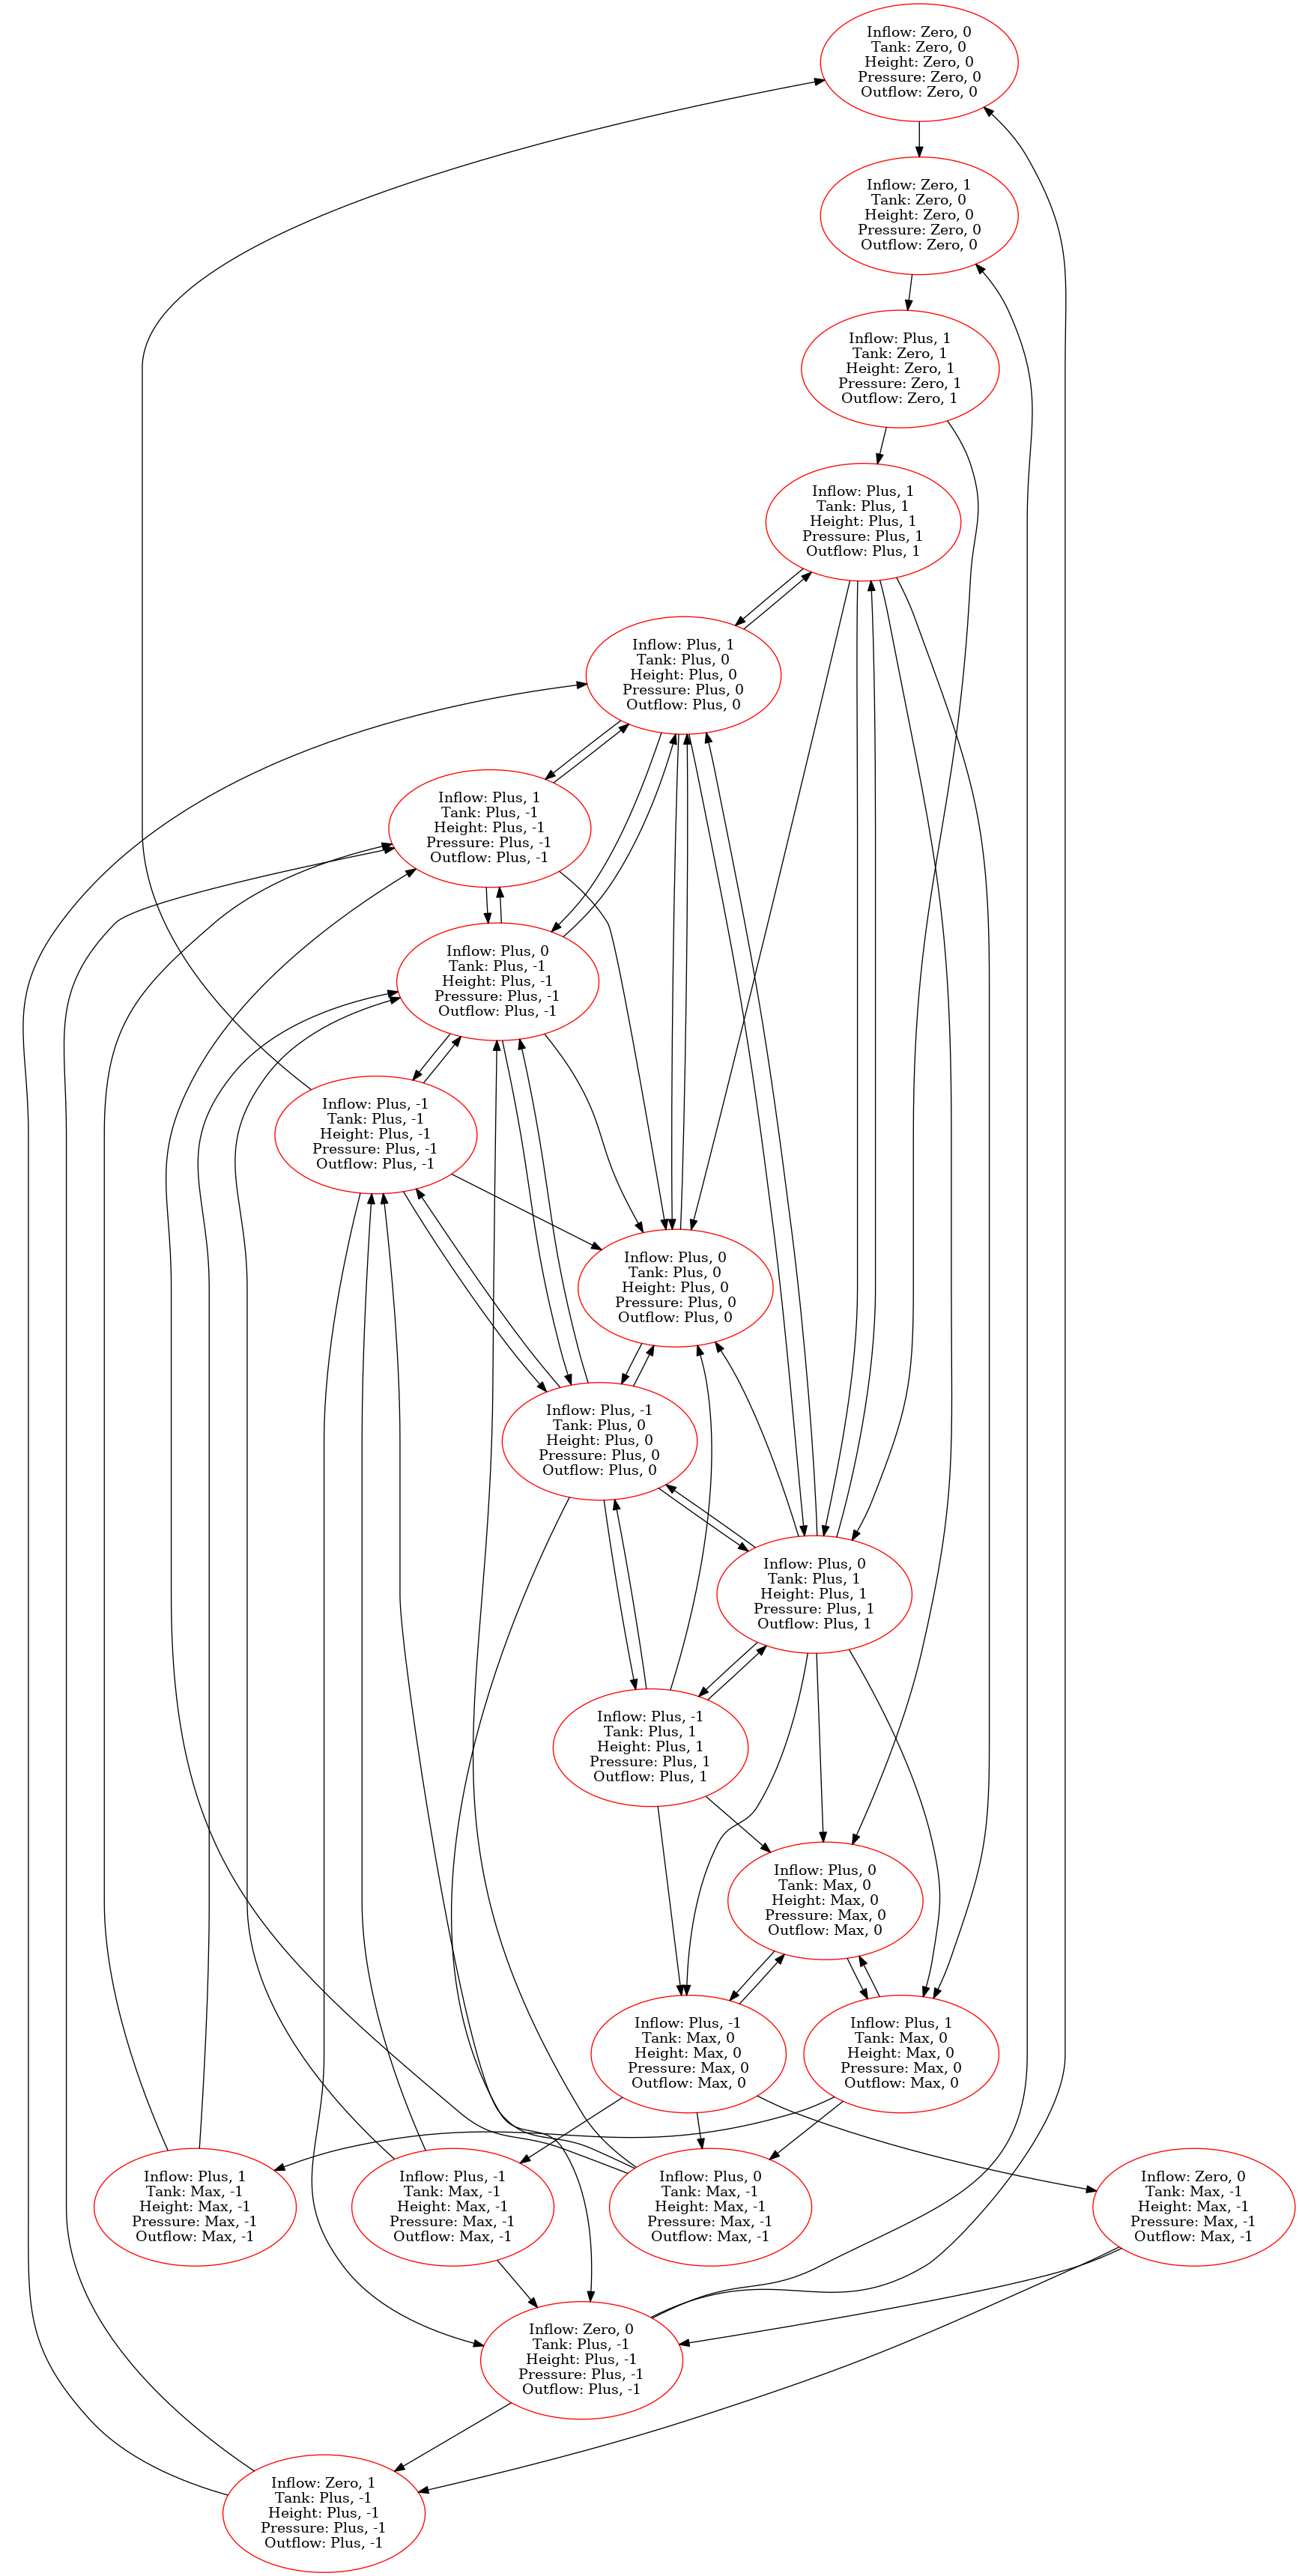
\includegraphics[width=\textwidth,height=\textheight,keepaspectratio]{result.png}
\caption{Plot of the state-graph}
\end{figure}

\section{Extra Problem}

\begin{itemize}
\item \textbf{Quantities:}
\begin{itemize}
\item Inflow (of water into the container) $\in [0, +]$
\item Outflow (of water out of the container) $\in [0, +, Max]$
\item Volume (of the water in the container) $\in [0, +, Max]$
\item Height (of the water column in the container) $\in [0, +, Max]$
\item Pressure (of the water column at the bottom of the container) $\in [0, +, Max]$
\end{itemize}

\item \textbf{Dependencies:}

\begin{itemize}
\item I+(Inflow, Volume): the amount of inflow increases the volume
\item I-(Outflow, Volume): the amount of outflow decreases the volume
\item P+(Volume, Height): height changes are proportional to volume changes
\item P+(Height, Pressure): pressure changes are proportional to height changes
\item P+(Pressure, Outflow): outflow changes are proportional to pressure changes
\item V(Volume(Max), Height(Max)): the height is at its highest value (Max), when the volume is at it highest value
\item V(Volume(0), Height(0)): there is no height, when there is no volume
\item V(Height(Max), Pressure(Max)): the pressure is at its highest value (Max), when the height is at it highest value
\item V(Height(0), Pressure(0)): there is no pressure, when there is no height
\item V(Pressure(Max), Outflow(Max)): the outflow is at its highest value (Max), when the pressure is at it highest value
\item V(Pressure(0), Outflow(0)): there is no outflow, when there is no pressure
\end{itemize}
\end{itemize}

\begin{figure}[H]
\centering
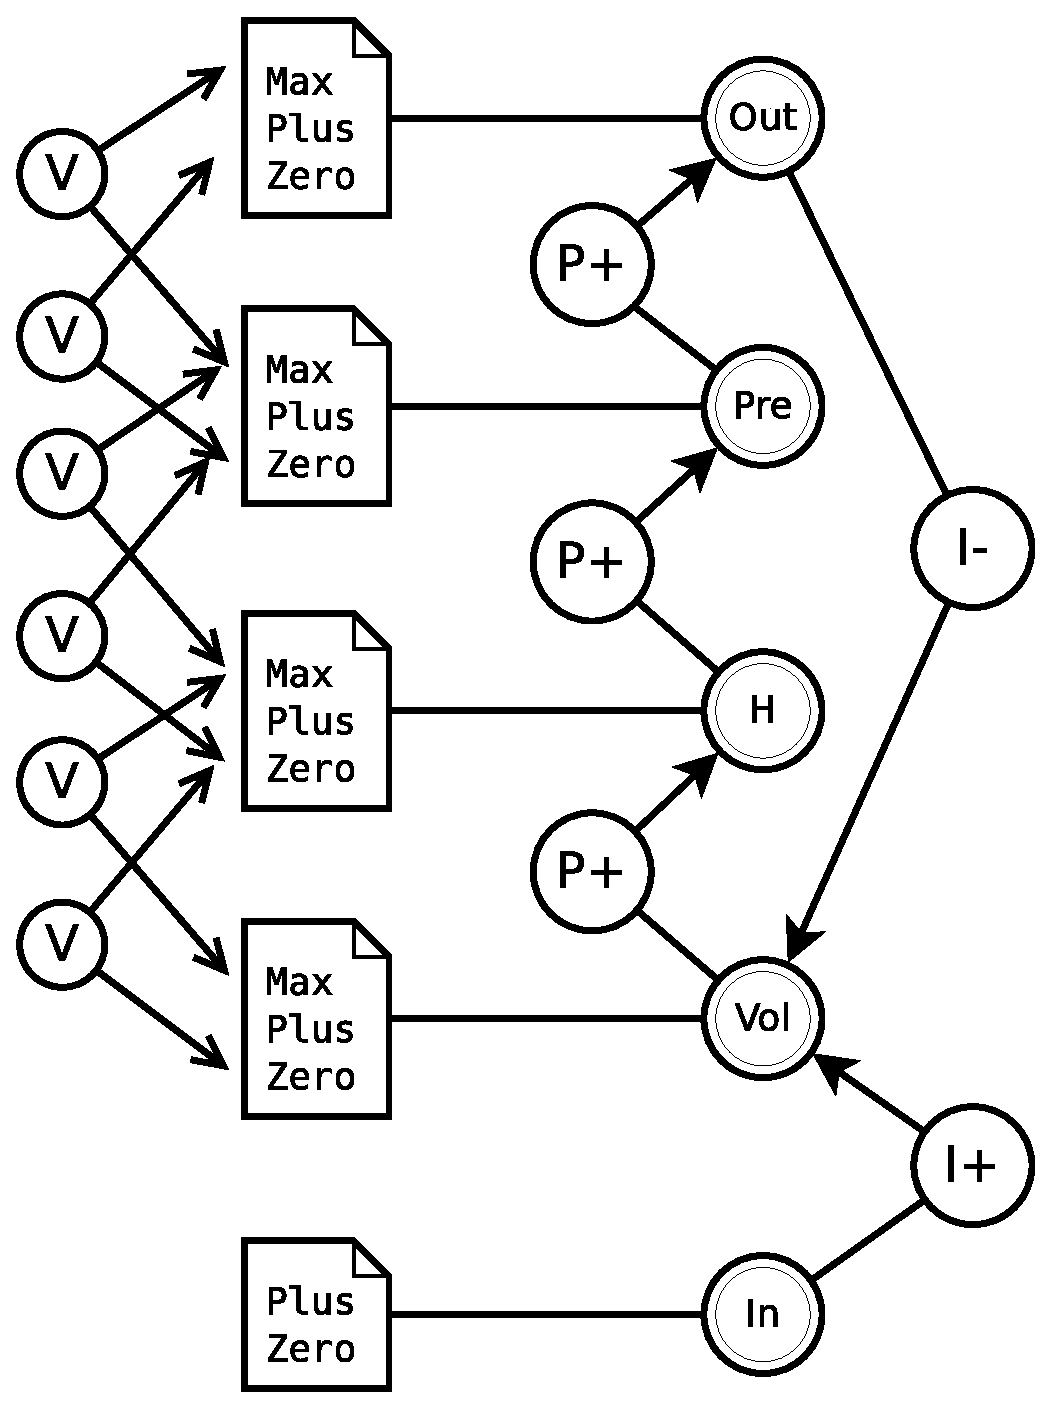
\includegraphics[scale=0.5]{problem_extra.eps}
\caption{Drawings of the causal model active for the extra problem}
\end{figure}


\end{document}

